\section{Modification des spécifications}
\subsection{Accessibilité du panneau d'interrupteurs}
A la suite d'une visite, nous avons confirmé avec nos clients de Kerpape qu'il était difficile d'accéder aux boutons du panneau de commandes dans l'application. A cause de leur taille, il fallait beaucoup de précision pour appuyer sur un bouton et non son voisin. Nous avons donc implémenté un système pour faciliter la visée de l'utilisateur en affichant les interrupteurs plus proches de la caméra.\newline

Lorsque l'utilisateur s'approche du panneau de commande, la caméra se déplace linéairement pour que les interrupteurs soient au centre de l'écran. De cette manière, les étiquettes sont plus visibles, et il est plus facile d'appuyer sur les boutons.\newline

A ce moment, les déplacements sont bloqués ainsi que la caméra. Lorsque l'utilisateur déplace la souris, le curseur se mouvoit de haut en bas et de gauche à droite. L'utilisateur peut ainsi actionner le bouton qu'il souhaite facilement. Pour sortir de ce mode bloqué, il faut appuyer sur la touche directionnelle bas ou 'S', comme pour s'éloigner du mur.

\begin{figure}[h]
	\centering
		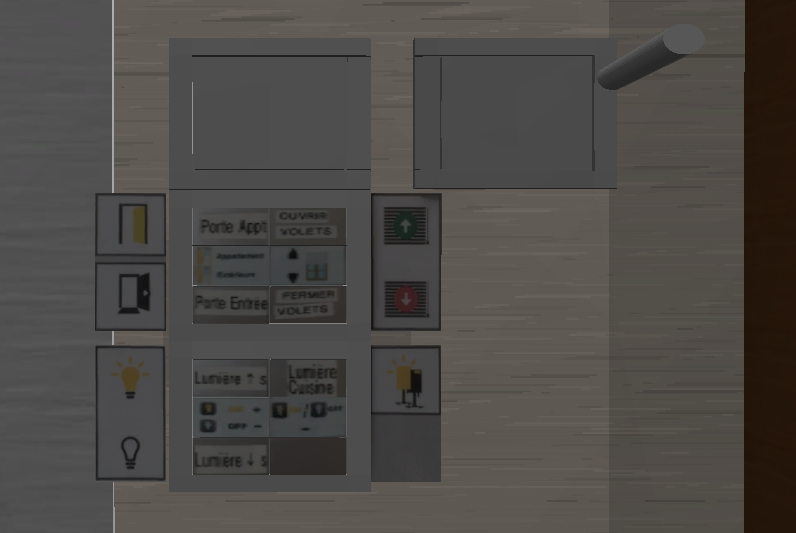
\includegraphics[width=\textwidth]{7-RapportFinal/img/screenshot_panneau_commande.png}
		\caption{Aperçu du panneau de commande dans l'application}
	\label{fig:panneau_commande}
\end{figure}
